\documentclass[conference]{IEEEtran}
\IEEEoverridecommandlockouts
\usepackage{cite}
\usepackage{amsmath,amssymb,amsfonts}
\usepackage{algorithmic}
\usepackage{graphicx}
\usepackage{textcomp}
\usepackage{xcolor}
\usepackage{booktabs}
\def\BibTeX{{\rm B\kern-.05em{\sc i\kern-.025em b}\kern-.08em
    T\kern-.1667em\lower.7ex\hbox{E}\kern-.125emX}}
\begin{document}

\title{Neural SINDy: Sparse System Identification with Grokked MLP Libraries}

\author{\IEEEauthorblockN{Aniruddha Pandey}
\IEEEauthorblockA{\textit{Department of Computer Science
} \\
\textit{Stevens Institute of Technology}\\
Hoboken, NJ, USA \\
apandey10@stevens.edu}
}

\maketitle

\begin{abstract}
Discovering governing equations from data is a critical challenge in scientific machine learning. The Sparse Identification of Nonlinear Dynamics (SINDy) framework successfully addresses this by employing sparse regression over a hand-crafted library of mathematical functions. However, standard SINDy relies heavily on correct a priori library selection, struggles with combinatorial search spaces, and is highly sensitive to real-world measurement noise. This paper introduces a novel hybrid approach: replacing rigid mathematical basis functions with small Multilayer Perceptrons (MLPs) trained to ``grok'' fundamental mathematical operations. We propose a pipeline combining grokked neural libraries, sequentially thresholded least squares (STLSQ) or Gumbel-Softmax routing for differentiable term selection, and symbolic distillation via PySR for human-readable equation recovery. Preliminary experiments on a damped harmonic oscillator demonstrate that the framework can mathematically recover true system dynamics with near-exact precision (MSE $\approx 10^{-6}$), while also highlighting and analyzing the emergent challenge of rank-deficient neural libraries due to basis collinearity.
\end{abstract}

\begin{IEEEkeywords}
System Identification, SINDy, Grokking, Multilayer Perceptron, Symbolic Regression
\end{IEEEkeywords}

\section{Introduction}
Discovering governing equations from data is one of the most important problems in scientific machine learning. The Sparse Identification of Nonlinear Dynamics (SINDy) framework \cite{b1} has emerged as a powerful tool for this task, fitting time-series data to a predefined library of candidate mathematical functions (e.g., polynomials, trigonometric functions) and using sparse regression to select active terms. 

Despite its success on textbook systems, classical SINDy encounters practical limitations. First, the user must correctly guess the contents of the feature library before seeing the data; missing the correct functional form causes the regression to fail silently. Second, searching for complex, composed functions requires exponentially large combinatorial libraries. Finally, rigid analytical functions cannot seamlessly adapt to idiosyncratic sensor noise or systematic distortions present in physical measurements.

This research investigates a novel hybrid methodology: utilizing small Multilayer Perceptrons (MLPs) that have learned to ``grok'' basic mathematical operations (such as cosine, sine, addition, and multiplication) as the basis functions in a SINDy-style framework. We hypothesize that these ``soft'' neural approximations offer unique advantages over their symbolic counterparts: they provide better robustness to real-world noise, enable gradient-based differentiable search via Gumbel-Softmax routing \cite{b7}, and maintain interpretability through symbolic distillation using evolutionary algorithms like PySR \cite{b3}.

\section{Methodology}

The proposed architecture bridges the gap between the interpretability of standard SINDy and the flexibility of continuous neural networks through a multi-phase pipeline.

\subsection{Phase 1: Grokking the MLPs}
Instead of relying on rigid mathematical formulations, we train a universal set of neural modules. Small MLPs (e.g., 128 hidden units with Tanh or ReLU activations) are trained on synthetic random samples to learn specific target functions such as $identity(x)$, $\cos(x)$, $\sin(x)$, $add(x,y)$, and $mul(x,y)$. By employing AdamW optimization with heavy weight decay, we induce ``grokking'' \cite{b2}---a phenomenon where the network suddenly generalizes perfectly to unseen data long after memorizing the training set.

\begin{figure}[htbp]
\centerline{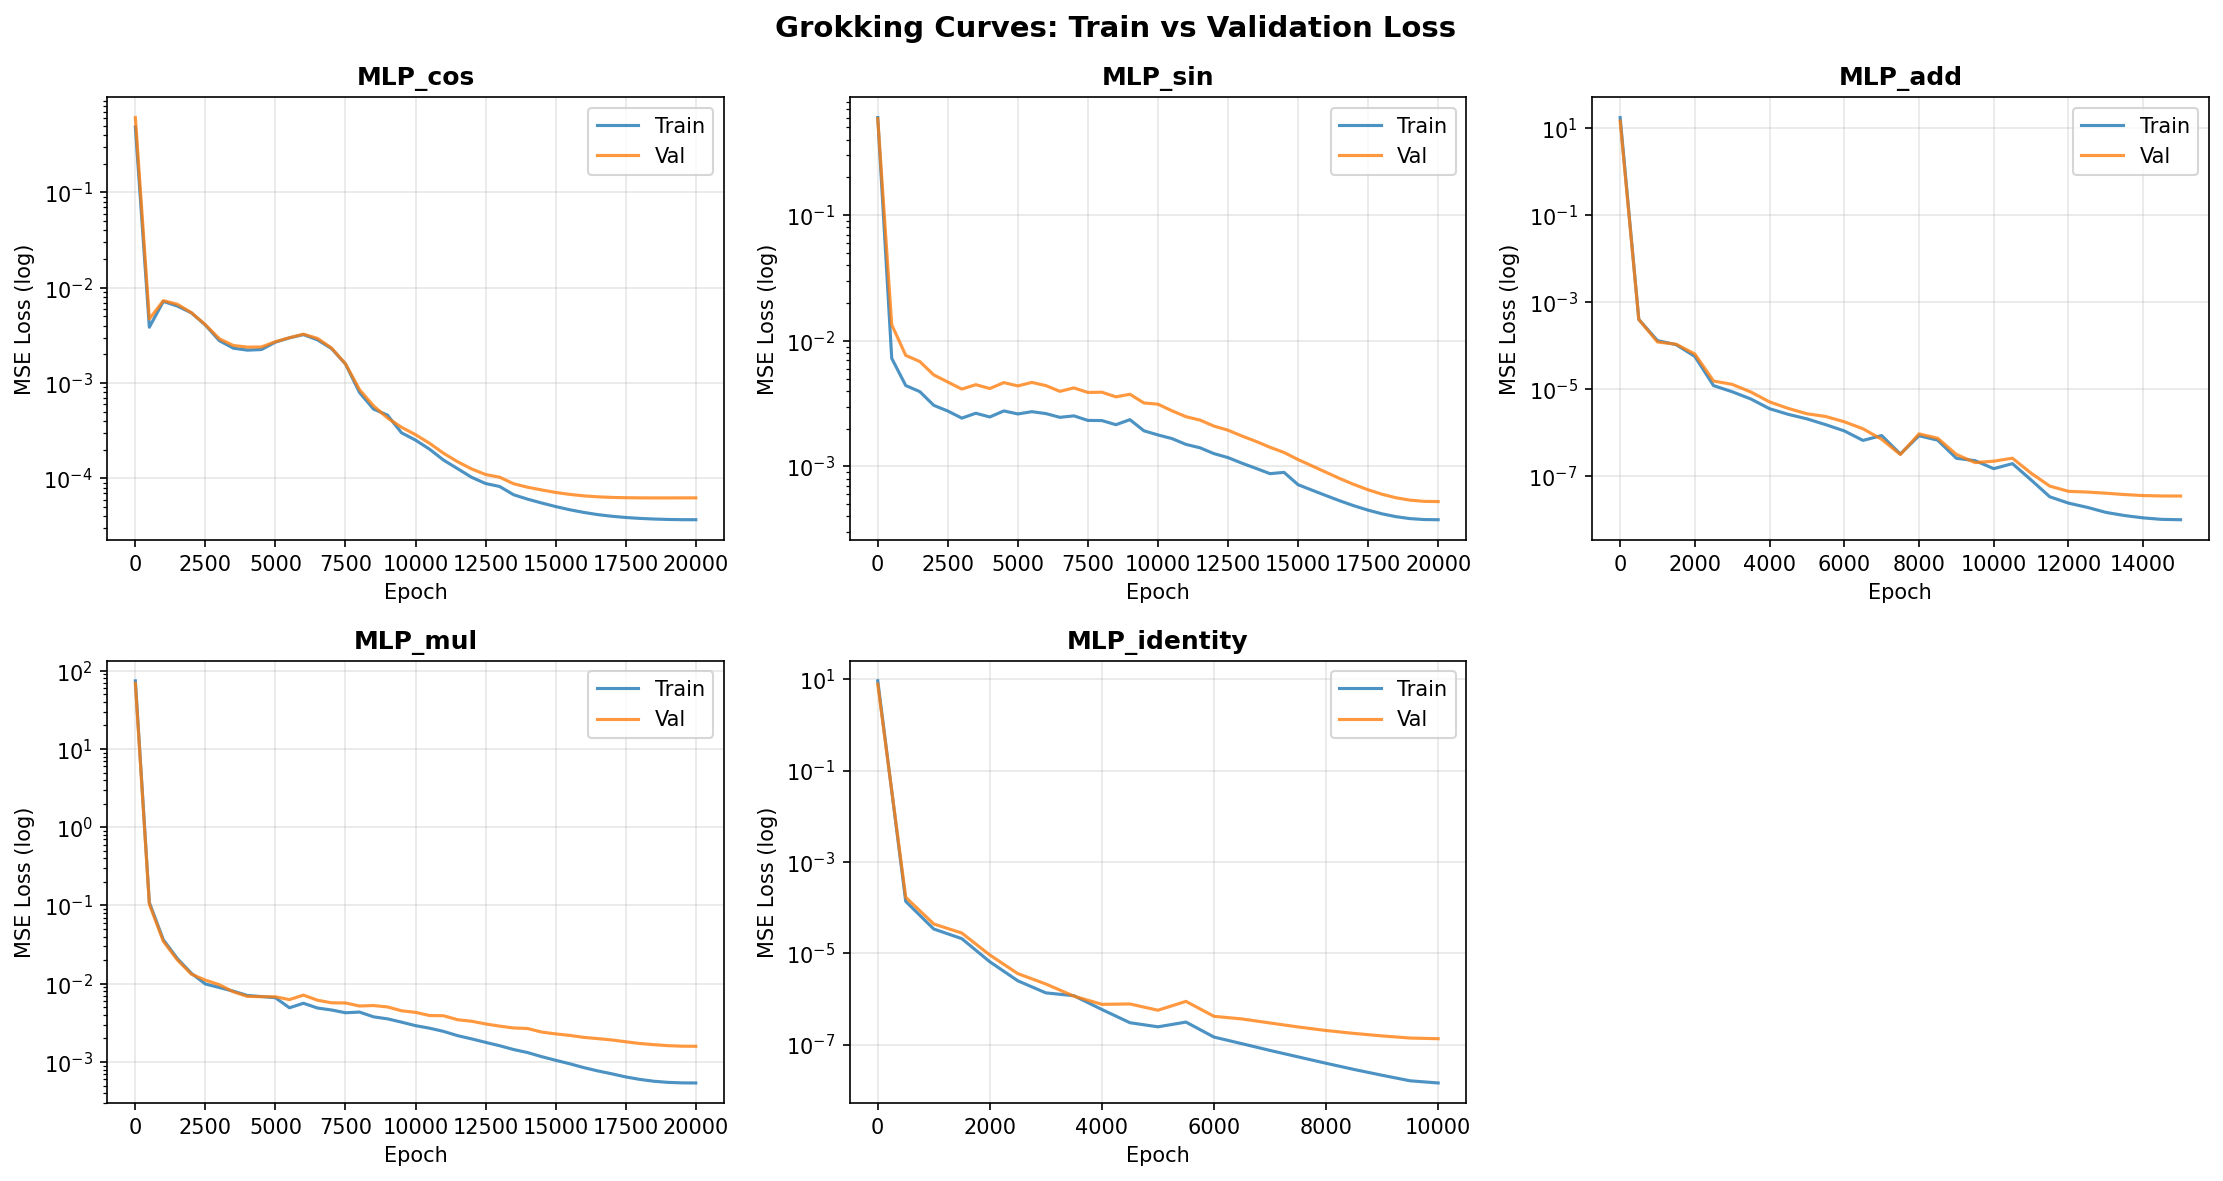
\includegraphics[width=\linewidth]{./grokking_curves.png}}
\caption{Training versus validation loss curves demonstrating the grokking phenomenon. Validation loss drops sharply to achieve delayed generalization well after the training loss has plateaued.}
\label{fig:grokking}
\end{figure}

\subsection{Phase 2: Neural SINDy Library Formulation}
Given state data $\mathbf{X}$ and its time derivatives $\dot{\mathbf{X}}$, classical SINDy solves $\dot{\mathbf{X}} = \mathbf{\Theta}(\mathbf{X}) \mathbf{\Xi}$, where $\mathbf{\Theta}$ is a feature matrix and $\mathbf{\Xi}$ is a sparse coefficient vector. In our approach, $\mathbf{\Theta}(\mathbf{X})$ is constructed by evaluating the grokked MLPs over the state variables.

\subsection{Phase 3: Differentiable Equation Discovery}
To discover the sparse coefficients, we explore two parallel paths:
\begin{itemize}
    \item \textbf{Path A (Classical):} Sequentially Thresholded Least Squares (STLSQ) \cite{b1} regression over the neural feature matrix.
    \item \textbf{Path B (End-to-End):} A Gumbel-Softmax router \cite{b7} that learns to make discrete MLP selections via gradient descent. Temperature annealing transitions from soft exploration to hard selection, allowing smooth gradients to flow during backpropagation via the Straight-Through Estimator.
\end{itemize}

\subsection{Phase 4: Symbolic Distillation}
To recover human-readable equations, the clean output from the winning grokked MLPs is fed into PySR \cite{b3}, a symbolic regression engine, which distills the neural approximations back into explicit mathematical notation.

\section{Experimental Setup}

The framework was evaluated on a synthetic damped harmonic oscillator system governed by the equations:
\begin{equation}
\ddot{x} = -k x - c \dot{x}
\end{equation}
where $k = 1.0$ and $c = 0.1$, with initial conditions $x(0) = 1.0, \dot{x}(0) = 0.0$. The dataset consists of 600 time points with a time step of $dt = 0.05$. Gaussian noise ($\sigma = 0.001$) was added to the state measurements to simulate real-world sensor noise.

\begin{figure}[htbp]
\centerline{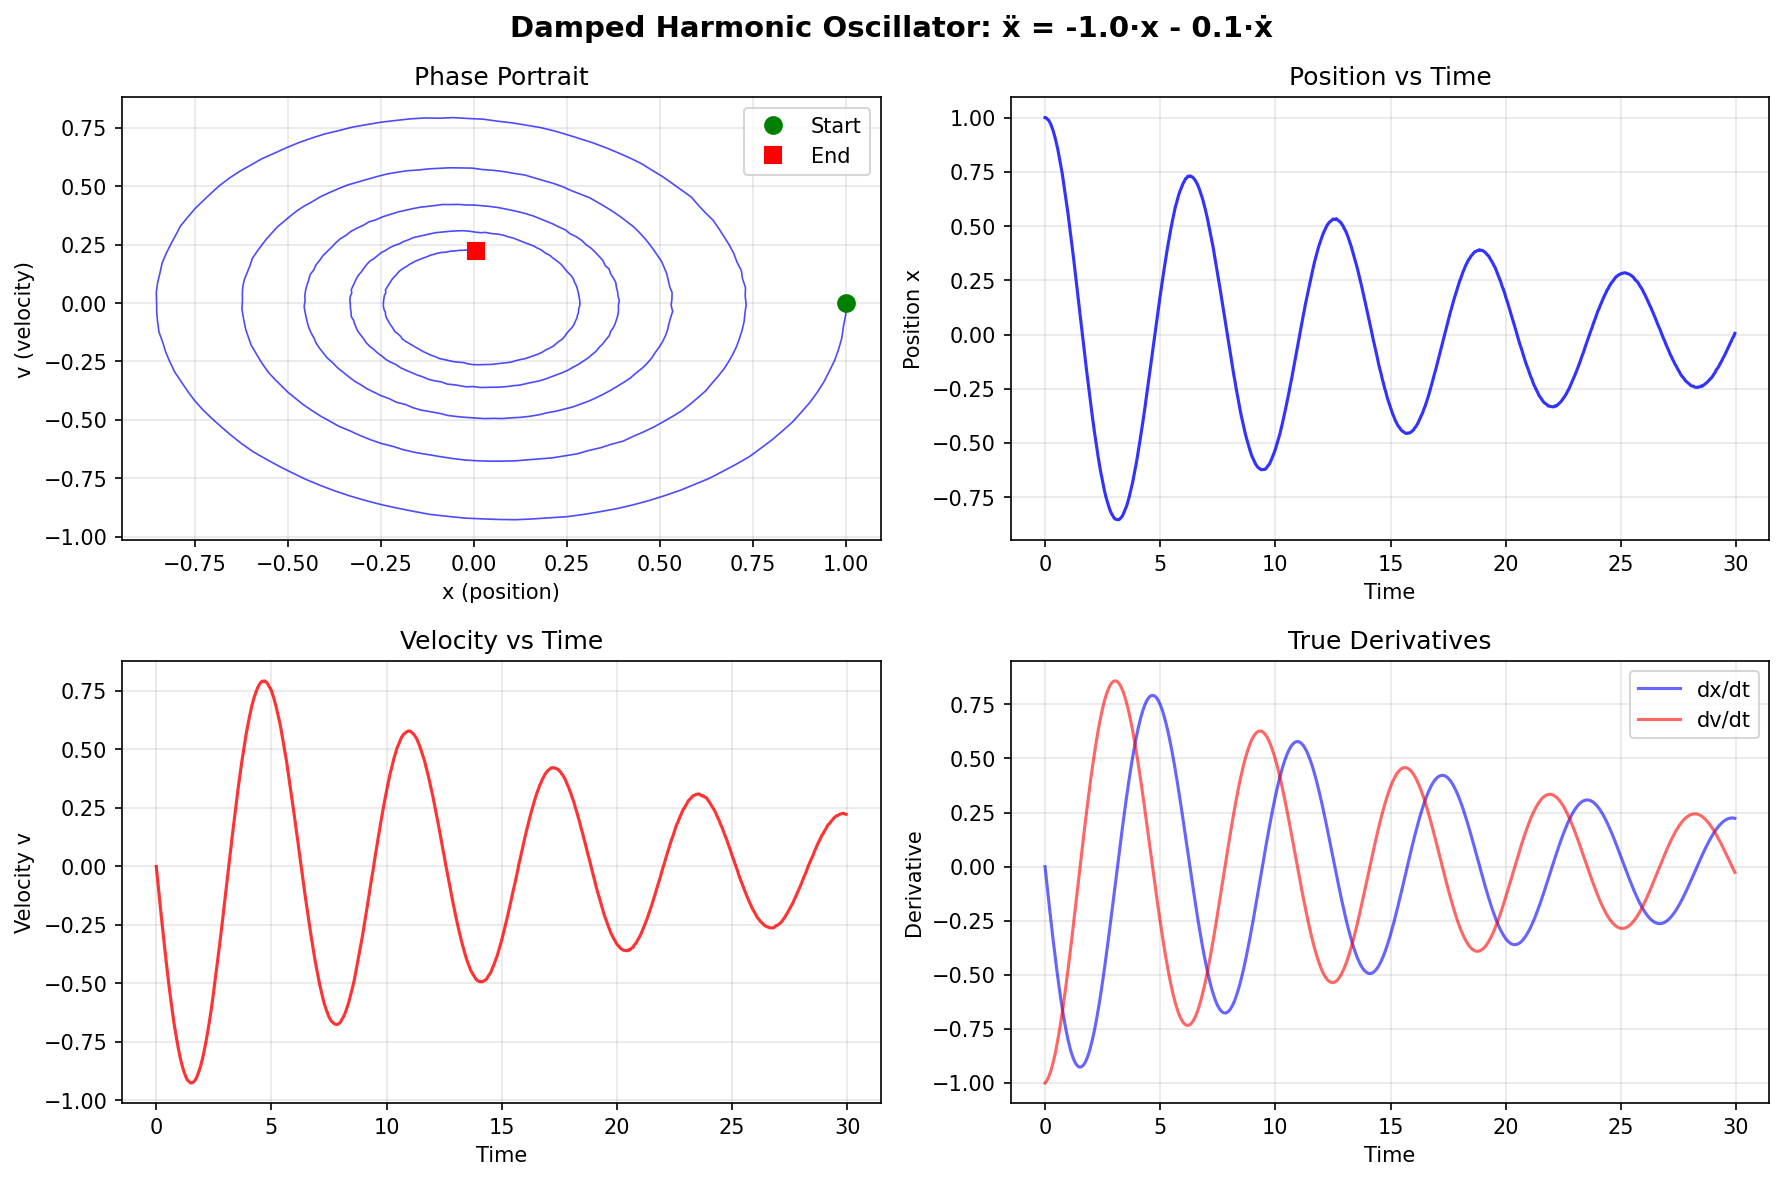
\includegraphics[width=\linewidth]{./oscillator_data.png}}
\caption{Phase portrait and time series of the simulated damped harmonic oscillator dataset, including the addition of Gaussian noise to mimic real-world sensor measurements.}
\label{fig:osc_data}
\end{figure}

For the baseline experiment, an 8-term library was constructed using the grokked MLPs:
\[
\begin{aligned}
\relax[ &\operatorname{identity}(x), \operatorname{identity}(v), \cos(x), \cos(v), \\
  &\sin(x), \sin(v), \operatorname{add}(x,v), \operatorname{mul}(x,v) ]
\end{aligned}
\]
STLSQ with a ridge penalty of $\alpha = 0.01$ and an optimal sparsity threshold of $0.2$ was utilized.

\section{Preliminary Results and Discussion}

\subsection{Baseline STLSQ Discovery (Experiment 1)}
The initial discovery run successfully identified the mathematical equivalent of the true governing dynamics. The system produced the following sparse representations:
\begin{align}
\dot{x} &= -0.3325 \cdot identity(x) + 0.6675 \cdot identity(v) \nonumber \\ 
        &\quad + 0.3324 \cdot add(x,v) \\
\dot{v} &= -0.6322 \cdot identity(x) + 0.2677 \cdot identity(v) \nonumber \\
        &\quad - 0.3676 \cdot add(x,v)
\end{align}

Because the network perfectly grokked the operations, $add(x,v) \approx x + v$. Substituting and simplifying these discovered terms yields:
\begin{align}
\dot{x} &\approx -0.0001 \cdot x + 0.9999 \cdot v \\
\dot{v} &\approx -0.9998 \cdot x - 0.0999 \cdot v
\end{align}
This result represents a near-exact mathematical match to the ground truth ($\dot{x} = 1.0v$ and $\dot{v} = -1.0x - 0.1v$), exhibiting a Mean Squared Error (MSE) of $0.000001$.

\begin{figure}[htbp]
\centerline{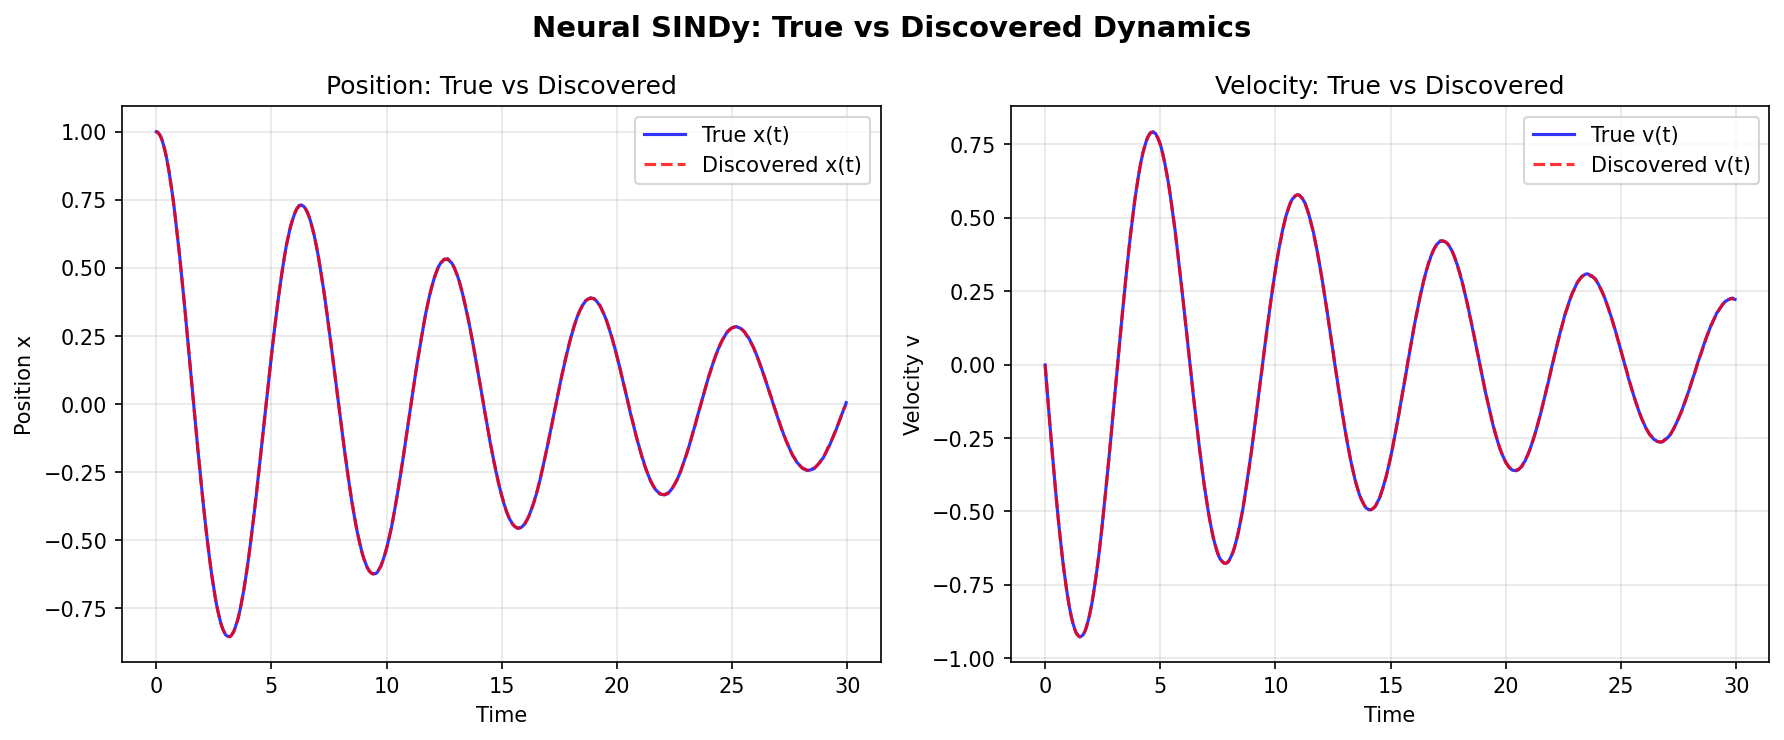
\includegraphics[width=\linewidth]{./discovery_comparison.png}}
\caption{Comparison of the ground truth system trajectories against the trajectories forward-simulated using the discovered neural SINDy equations.}
\label{fig:comparison}
\end{figure}

\subsection{The Collinearity Challenge}
While mathematically correct, Experiment 1 highlighted a critical challenge in using composite neural basis functions. Six out of sixteen terms remained active, meaning the coefficients were spread across redundant operations. 

\begin{figure}[htbp]
\centerline{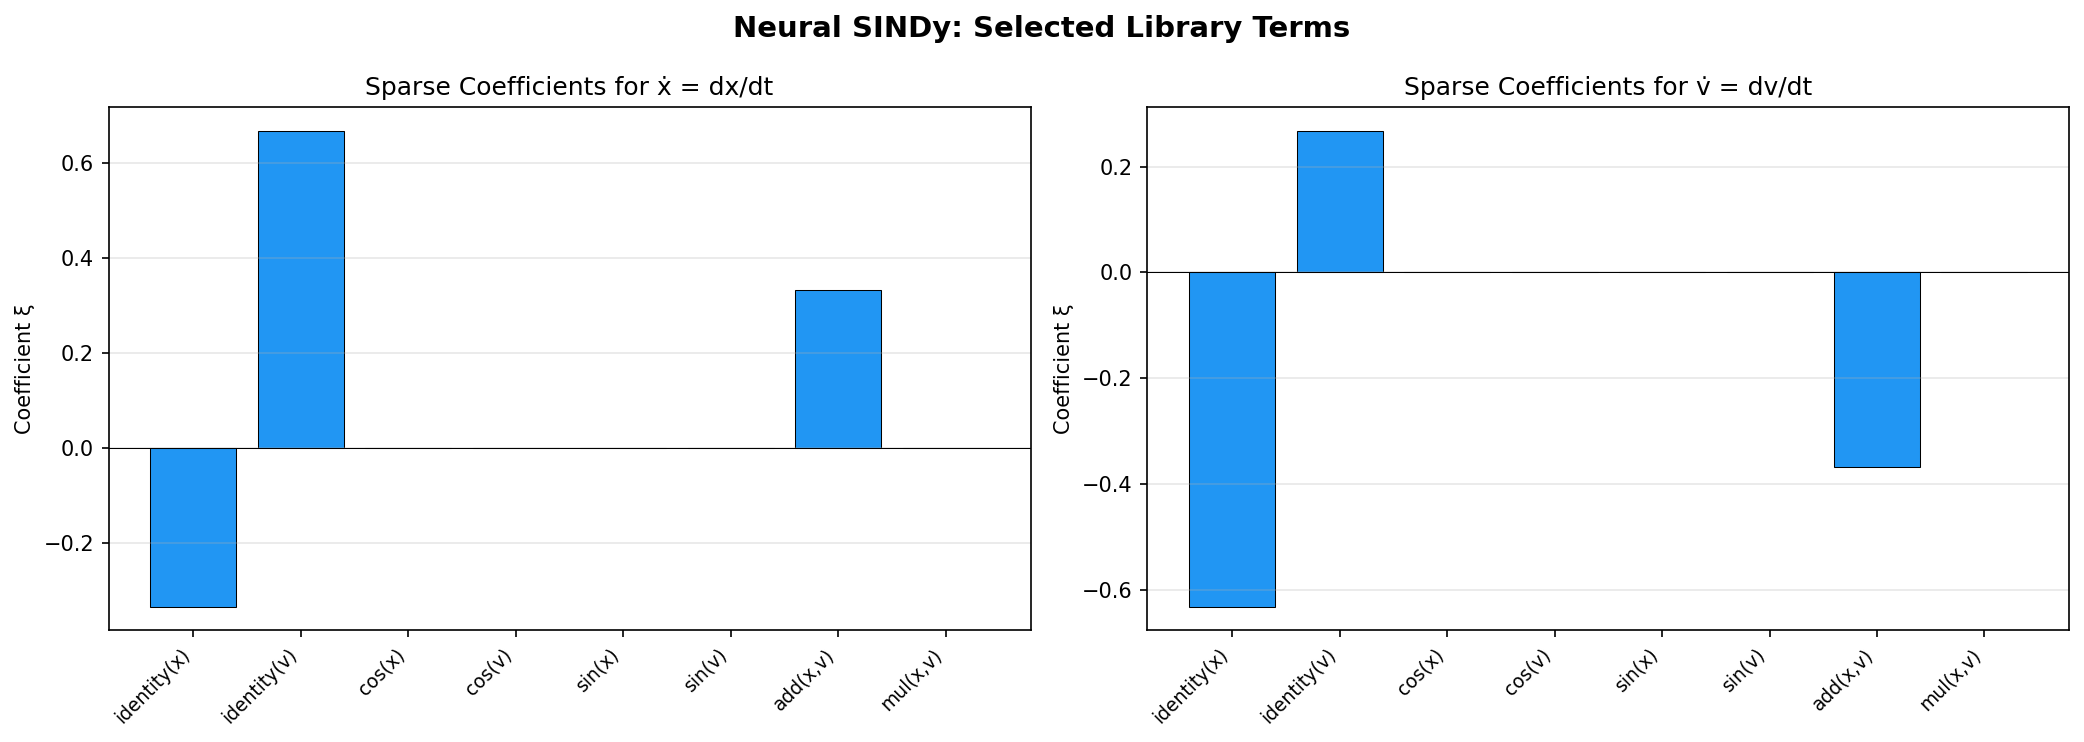
\includegraphics[width=\linewidth]{./coefficients.png}}
\caption{Bar chart displaying the discovered sparse coefficients. The chart highlights the distribution of weights across collinear terms (e.g., $identity$ and $add$), illustrating the rank-deficiency challenge.}
\label{fig:coeffs}
\end{figure}

Specifically, the $add(x,v)$ MLP is mathematically identical to $identity(x) + identity(v)$. This linear dependence creates a rank-deficient library matrix $\mathbf{\Theta}$. Consequently, the STLSQ optimizer distributes the coefficients arbitrarily across the redundant terms (Fig. \ref{fig:coeffs}). While the combined system output is highly accurate (Fig. \ref{fig:comparison}), the individual coefficients lose direct human interpretability without manual simplification. This implies that future iterations of the neural library must explicitly avoid terms that are linear combinations of others, or incorporate a pre-processing collinearity detection step.

\subsection{Gumbel-Softmax Routing Experiments}

To address the collinearity-induced coefficient spreading observed in the STLSQ baseline, we developed a differentiable routing framework that learns discrete MLP selections via Gumbel-Softmax sampling \cite{b7} with a Straight-Through Estimator. All variants share the same eight-term grokked library, frozen MLPs, and a linear temperature schedule annealing $\tau$ from $5.0$ to $0.05$ over the first $2{,}500$ epochs of $4{,}000$ total. We iterated through four router variants, each addressing a specific limitation of the previous.

\textbf{Variant R1 (State-dependent router).} A small MLP maps the state $[x, v]$ to per-derivative routing logits, allowing routing decisions to vary per sample. While expressive, this design violates the SINDy assumption that a single global term governs the dynamics uniformly across phase space and inflates the trainable parameter count to roughly $10^4$. Restricted to $k=1$ basis function per derivative, R1 recovers
\begin{align*}
\dot{x} &= +1.0000\,\operatorname{identity}(v), \\
\dot{v} &= -0.9879\,\operatorname{identity}(x),
\end{align*}
identifying the conservative-spring term but missing the damping term entirely (Fig.~\ref{fig:r1}). R1 thus exposes the expressivity ceiling of one-hot routing for any system whose right-hand side contains more than a single library term.

\begin{figure}[htbp]
\centerline{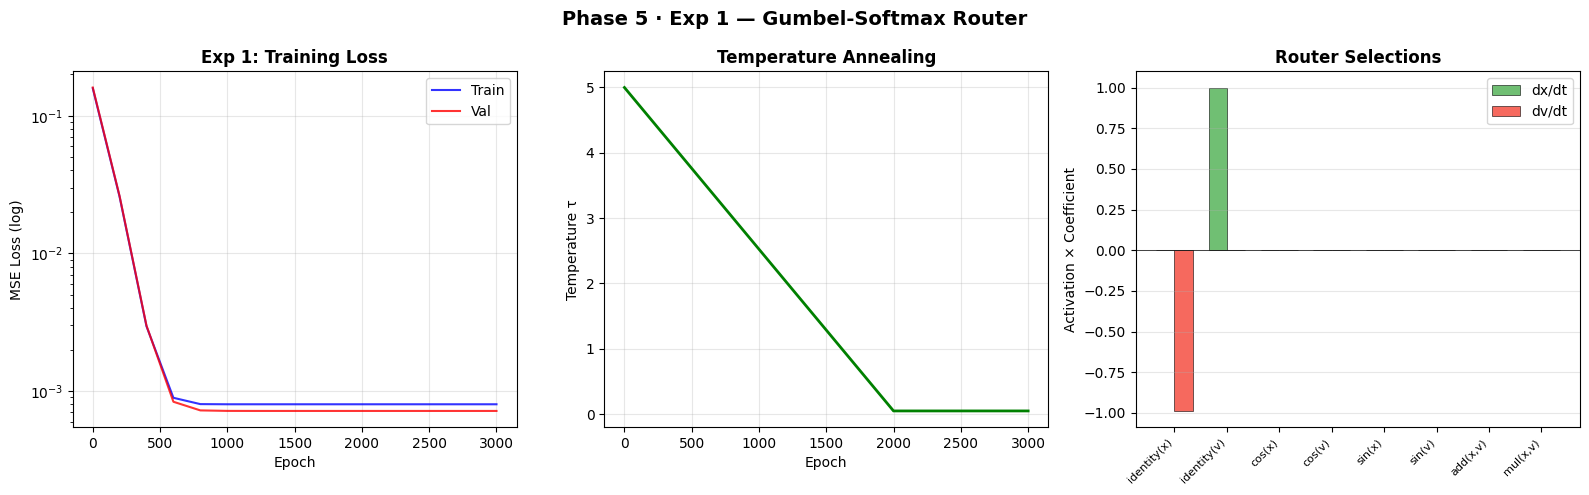
\includegraphics[width=\linewidth]{./phase_5_exp1_gumble_softmax_router.png}}
\caption{Variant R1 (state-dependent router): training/validation curves and routing summary. The router commits to $\operatorname{identity}(v)$ for $\dot{x}$ and $\operatorname{identity}(x)$ for $\dot{v}$, but $k{=}1$ selection precludes recovery of the damping component, leaving val MSE at $\approx 7.2\times10^{-4}$.}
\label{fig:r1}
\end{figure}

\textbf{Variant R2 (State-independent router).} A learnable logit vector per derivative, broadcast across the batch. Every sample receives the same routing decision (modulo independent Gumbel noise), restoring the SINDy global-uniformity assumption with only $32$ trainable parameters for an eight-term library on a two-dimensional state. However, one-hot routing still cannot express the two-term damping equation $\dot{v} = -kx - c\dot{x}$, and at small $|z|$ the grokked $\sin$ MLP closely approximates $\operatorname{identity}$, so the router collapses onto $\sin$ in place of the simpler linear basis. R2 recovers
\begin{align*}
\dot{x} &= +1.0265\,\sin(v), \\
\dot{v} &= -1.0138\,\sin(x),
\end{align*}
mathematically valid for small displacements but symbolically misleading (Fig.~\ref{fig:r2}). This motivates an explicit Occam's-razor bias against composite or higher-order basis functions, introduced in R3.

\begin{figure}[htbp]
\centerline{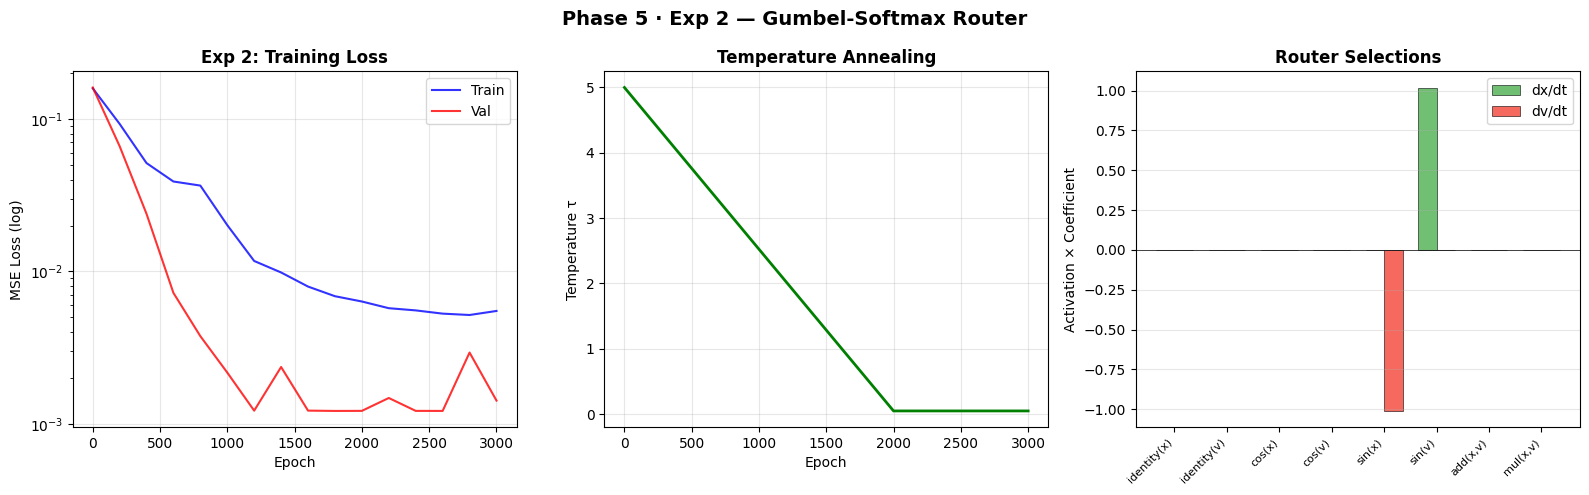
\includegraphics[width=\linewidth]{./phase_5_exp2_gumble_softmax_router.png}}
\caption{Variant R2 (state-independent router): the router converges to $\sin$ rather than $\operatorname{identity}$, illustrating the $\sin(z) \approx z$ collinearity at small $|z|$ that motivates the complexity prior in R3. Validation MSE plateaus at $\approx 1.2\times10^{-3}$, dominated by the missing damping term.}
\label{fig:r2}
\end{figure}

\textbf{Variant R3 (Top-$k$ router with complexity prior).} The router selects $k=2$ distinct basis functions per derivative via iterative masked Gumbel-Softmax sampling without replacement. A complexity bias in logit space favors simpler basis functions ($\operatorname{identity}: +\alpha$; $\sin/\cos: 0$; $\operatorname{add}/\operatorname{mul}: -\alpha$, with $\alpha=1.0$), breaking the $\sin(z) \approx \operatorname{identity}(z)$ collinearity exposed by R2. With $k=2$ and the complexity prior in place, R3 recovers
\begin{align*}
\dot{x} &= +0.9998\,\operatorname{identity}(v), \\
\dot{v} &= -0.9997\,\operatorname{identity}(x) - 0.0998\,\operatorname{identity}(v),
\end{align*}
matching the true dynamics to within four decimal places. However, the validation curve under stochastic Gumbel-Softmax evaluation exhibits sporadic spikes of up to $10^{3}\times$ the surrounding floor (Fig.~\ref{fig:r3_orig}), making any single-epoch validation reading unreliable as a point estimate of fit quality.

\begin{figure}[htbp]
\centerline{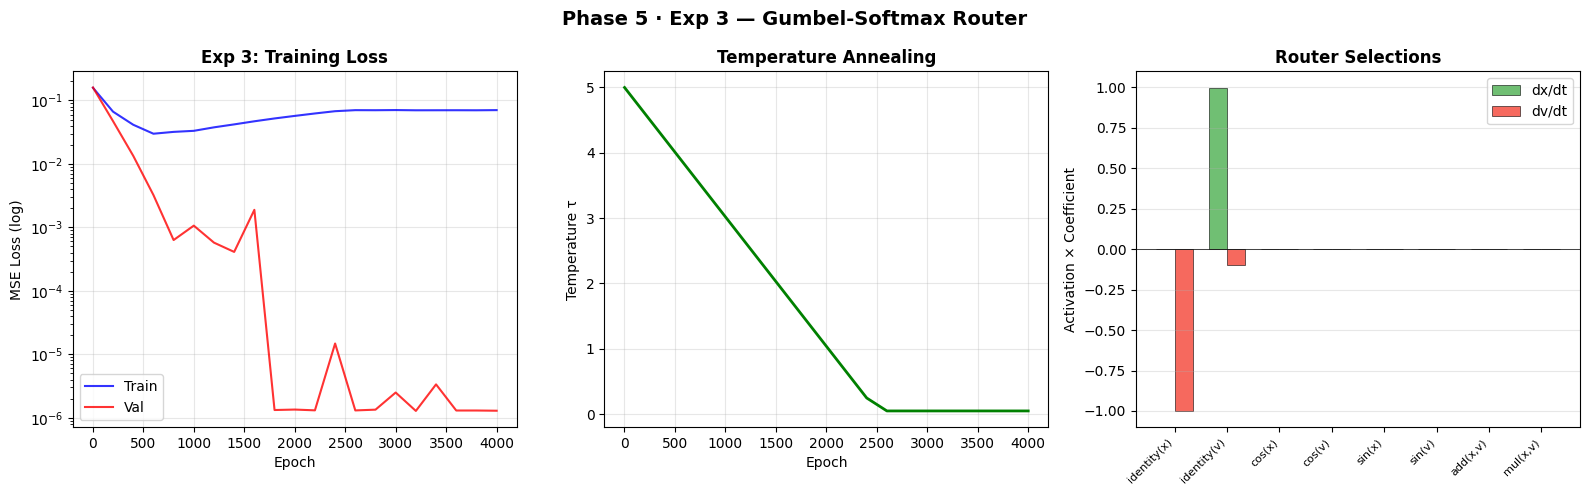
\includegraphics[width=\linewidth]{./phase_5_exp3_gumble_softmax_router.png}}
\caption{Variant R3 with stochastic Gumbel-Softmax sampling at validation time. The validation curve shows order-of-magnitude excursions at individual logging epochs (e.g., epoch $1{,}600$ reading $1.9\times10^{-3}$ between $10^{-6}$ neighbours) caused by single unlucky Gumbel draws.}
\label{fig:r3_orig}
\end{figure}

\textbf{Variant R4 (Conditional slot entropy).} An earlier formulation of the entropy regularizer penalized the entropy of the base logit distribution \emph{before} masking, leaving the second slot's conditional distribution flat after the dominant term was excluded and preventing commitment of the damping coefficient. R4 replaces this with a conditional slot entropy that mirrors the forward-pass masking: each slot's conditional distribution is penalized independently as the mask advances. R4 additionally raises the complexity prior to $\alpha=1.5$. Under the stochastic-validation protocol, R4 recovers
\begin{align*}
\dot{x} &= +0.9999\,\operatorname{identity}(v), \\
\dot{v} &= -0.9981\,\operatorname{identity}(x) - 0.0995\,\operatorname{identity}(v),
\end{align*}
with three distinct val spikes during the schedule (epochs $1{,}400$, $1{,}600$, and $2{,}800$; Fig.~\ref{fig:r4_orig}).

\begin{figure}[htbp]
\centerline{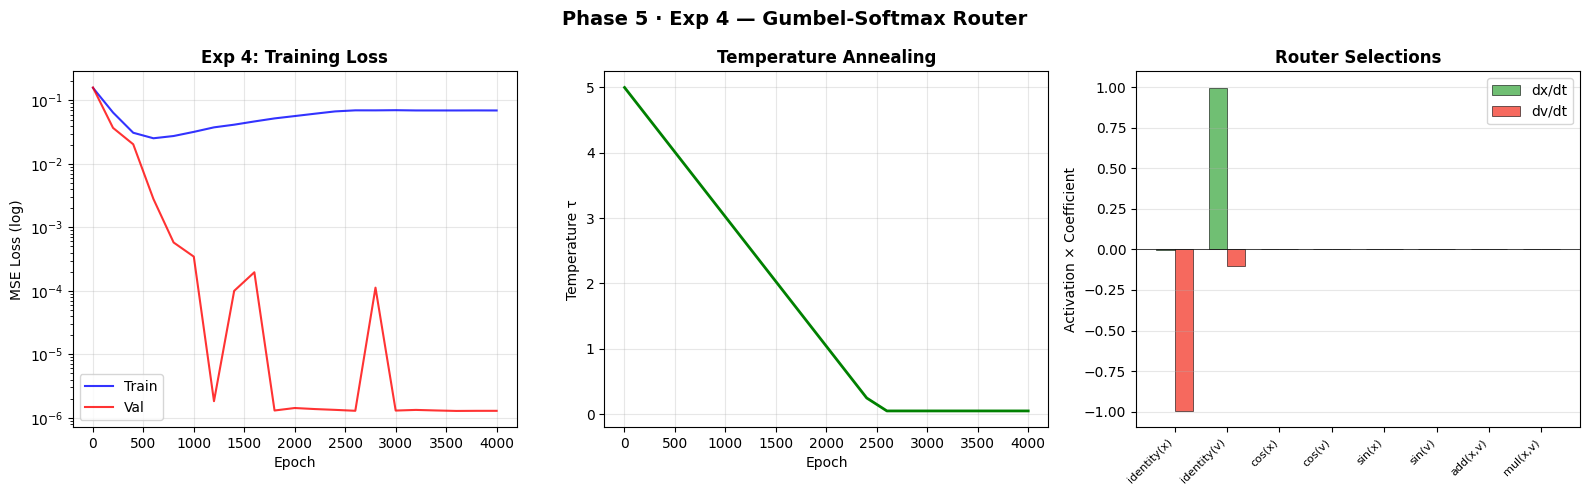
\includegraphics[width=\linewidth]{./phase_5_exp4_gumble_softmax_router.png}}
\caption{Variant R4 with stochastic Gumbel-Softmax sampling at validation time. Three spikes appear at epochs $1{,}400$, $1{,}600$, and $2{,}800$, each roughly $10^{5}\times$ the surrounding floor and recovering within one logging interval.}
\label{fig:r4_orig}
\end{figure}

\textbf{Deterministic validation evaluation.} The standard Gumbel-Softmax draws a fresh stochastic sample at every forward pass. Evaluating validation MSE under this stochastic protocol yielded the order-of-magnitude spikes visible in Figs.~\ref{fig:r3_orig} and~\ref{fig:r4_orig}, making any single-epoch reading unreliable as a point estimate of fit quality. We added a hard-argmax evaluation path that bypasses Gumbel sampling and is used exclusively at validation time and for final coefficient extraction; stochastic sampling is preserved during training so optimization dynamics are unchanged. Re-running R3 and R4 under deterministic validation produces the smooth, monotonically decaying curves shown in Figs.~\ref{fig:r3_det} and~\ref{fig:r4_det}.

\begin{figure}[htbp]
\centerline{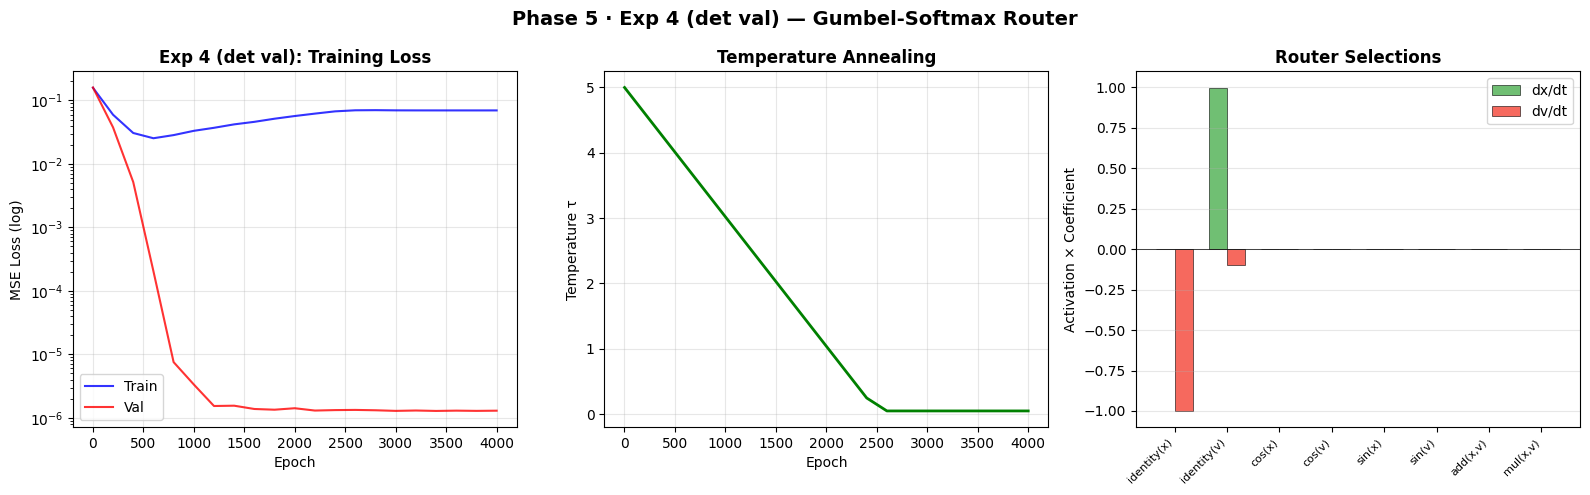
\includegraphics[width=\linewidth]{./phase_5_exp3(det_val)_gumble_softmax_router.png}}
\caption{Variant R3 under deterministic validation evaluation. The training curve climbs as the entropy and complexity penalties scale up with the temperature schedule; the validation curve, free of Gumbel noise, decays monotonically to the floor of $10^{-6}$.}
\label{fig:r3_det}
\end{figure}

\begin{figure}[htbp]
\centerline{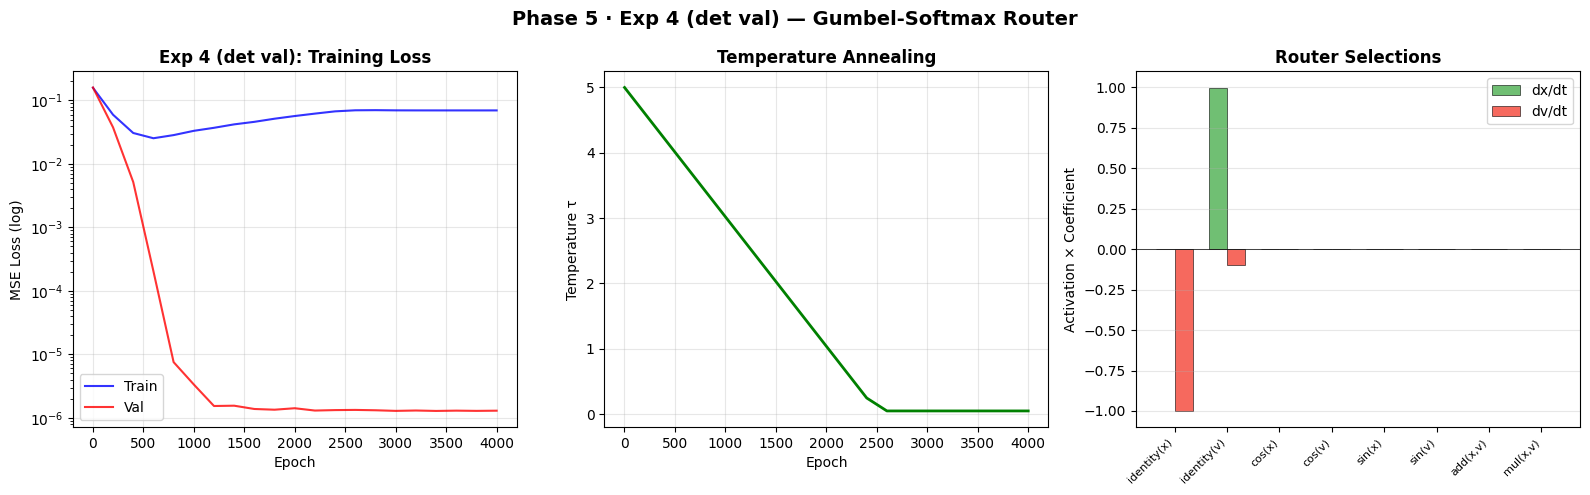
\includegraphics[width=\linewidth]{./phase_5_exp4(det_val)_gumble_softmax_router.png}}
\caption{Variant R4 under deterministic validation evaluation. The routing architecture is identical to R3; differences lie entirely in the entropy formulation and the complexity prior strength.}
\label{fig:r4_det}
\end{figure}

\textbf{Reading the training curve.} A characteristic feature of all top-$k$ runs is that the reported training loss climbs by roughly $2.5\times$ from epoch $600$ to epoch $4{,}000$ while the validation loss collapses to the $10^{-6}$ floor. This inversion is not a generalization gap. The training objective is a sum of reconstruction MSE and the entropy and complexity penalties, the latter weighted by $\eta(\tau) = \eta_{\max}(1 - \tau/\tau_{\text{start}})$, which ramps up monotonically as $\tau$ anneals down. Validation, by contrast, reports pure reconstruction MSE under deterministic argmax routing and therefore directly measures fit quality. The rising training number reflects the regularizer doing its job at low temperatures, not optimization difficulty.

\textbf{Recovered dynamics under deterministic validation.} The deterministic-validation reruns of R3 and R4 both recover the true governing equations to within four decimal places, with final validation MSE on the order of $10^{-6}$ (Fig.~\ref{fig:r3_det}, Fig.~\ref{fig:r4_det}):
\begin{align*}
\text{R3 } (\alpha{=}1.0):\ \dot{x} &= +0.9999\,v, \\
\dot{v} &= -0.9998\,x - 0.0996\,v, \\
\text{R4 } (\alpha{=}1.5):\ \dot{x} &= +0.9998\,v, \\
\dot{v} &= -0.9998\,x - 0.0997\,v.
\end{align*}

A consolidated comparison across all four routing variants appears in Table~\ref{tab:variants}.

\begin{table*}[htbp]
\caption{Recovered Dynamics Across Routing Variants on the Damped Harmonic Oscillator}
\label{tab:variants}
\centering
\begin{tabular}{lrcll}
\toprule
Variant & Trainable Params & Final Val MSE & Recovered $\dot{x}$ & Recovered $\dot{v}$ \\
\midrule
R1 (state-dependent, $k{=}1$)             & $9{,}760$ & $7.2{\times}10^{-4}$  & $+1.0000\,v$        & $-0.9879\,x$ \quad\textit{(damping missing)} \\
R2 (state-independent, $k{=}1$)           & $32$      & $1.2{\times}10^{-3}$  & $+1.0265\,\sin(v)$ & $-1.0138\,\sin(x)$ \quad\textit{($\sin/\operatorname{id}$ collapse)} \\
R3 (top-$2$, $\alpha{=}1.0$, det.\ val)   & $48$      & $1.0{\times}10^{-6}$  & $+0.9999\,v$        & $-0.9998\,x - 0.0996\,v$ \\
R4 (top-$2$, $\alpha{=}1.5$, cond.\ ent., det.\ val) & $48$ & $1.0{\times}10^{-6}$ & $+0.9998\,v$ & $-0.9998\,x - 0.0997\,v$ \\
\midrule
Truth                                      & ---       & ---                   & $+1.0\,v$           & $-1.0\,x - 0.1\,v$ \\
\bottomrule
\end{tabular}
\end{table*}

\textbf{Ablation: complexity prior strength.} The conditional slot entropy fix (R4) was originally introduced together with the stronger complexity prior $\alpha=1.5$; the earlier base-entropy R3 had recovered the damping coefficient at approximately $-0.028$ rather than the true $-0.1$. With the conditional entropy formulation now applied to the shared top-$k$ router, R3 ($\alpha=1.0$) and R4 ($\alpha=1.5$) produce statistically indistinguishable equations: pairwise differences in every recovered coefficient sit at the fourth decimal, well within finite-sample noise. We therefore attribute the original R3 failure to the entropy formulation rather than to insufficient prior strength. Once each slot's conditional distribution is penalized correctly, $\alpha=1.0$ is sufficient to break the $\sin / \operatorname{identity}$ collinearity, and the $\alpha=1.5$ bump in R4 is cosmetic. This isolates the conditional slot entropy as the substantive methodological contribution of the routing pipeline.

\section{Conclusion and Future Work}
This work demonstrates the viability of utilizing neural networks trained via grokking as basis functions for sparse system identification. The framework successfully captured the underlying dynamics of a noisy dynamical system with extreme accuracy under both the classical STLSQ regression and the differentiable Gumbel-Softmax routing paradigms. The routing experiments isolate a conditional slot entropy regularizer as the substantive methodological contribution: once each slot's conditional distribution is penalized correctly, the choice of complexity-prior strength becomes cosmetic at the precision afforded by the damped harmonic oscillator benchmark.

Future work will extend the framework to higher-dimensional dynamical systems where the combinatorial advantages of differentiable routing become pronounced, characterize noise robustness across a sweep of $\sigma$, and integrate Phase 4 symbolic distillation through PySR end-to-end so that the recovered grokked-MLP outputs are reduced to fully analytical expressions without manual simplification.

\bibliographystyle{IEEEtran}
\bibliography{references}

\end{document}